\chapter{Algorithmic Specification Language}
\label{ch:al}
\noindent


SpecTec introduces AL, an algorithmic specification language, for specifying
the prose specification.
Since the prose notation of the official specification is informal, it is
essential to rigorously define AL to ensure an unambiguous and correct
specification, rather than merely imitating the original.
We begin by outlining the ambiguity of the prose specification in
\cref{sec:prose-informal}.
Next, we propose a formal model for Wasm control flow in AL in
\cref{sec:model}.
We then define the syntax and the semantics of AL in \cref{sec:definition}.
Finally, we produce an executable Wasm specification using AL interpreter that
ensures the correctness of the specification in \cref{sec:exec-spec}.

\section{Ambiguity in the prose specification}
\label{sec:prose-informal}

The prose specification describes Wasm semantics in an informal manner,
particularly when addressing control flow.
% Jump
Wasm control instructions \textit{jump} to certain code point for control
transfer.
While it does not explicitly explain the mechanics of jumping, the simplest
interpretation involves assuming a program counter.
\cref{fig:return} illustrates the prose specification for the \texttt{return}
instruction.
In the final step, it jumps to the instruction after the original call that
pushed the frame, which likely corresponds to updating the program counter to
the return address stored in the frame.


% Execute
On the other hand, some control instructions \textit{execute} a Wasm
instruction.
\cref{fig:if} represents the prose specification for the \texttt{if}
instruction, which executes a block instruction with instructions in the then
branch or the else branch based on the value in the stack.
However, the block instruction itself does not appeared in the actual code,
making its execution unclear in this context.
The situation become even more complicated when the block contains control
instructions, such as function call.
While the intended meaning can still be inferred, this informality introduces
ambiguity, leaving room for multiple interpretations.


\section{A Formal Model for WebAssembly Control Flow}
\label{sec:model}


% TODO: Clever way to distinguish jargon rather then \textit
% Formal model
To formally specify the prose specification, we construct a formal model to
describe Wasm control flow.
% Execute
Rather than relying on a program counter, we employ an instruction stack to
represent execution progress.
Execution proceeds by popping an instruction from the stack and performing its
operation.
To avoid confusion with the stack that contains values interleaved with
contexts, we refer to the latter as the \textit{interleaved stack}.
This approach allows us to define the execute operation without introducing a
program counter.


% Jump
We then split two distinct usages of the jump operation: \textit{enter} and
\textit{exit}.
Since Wasm supports structured control flow, the jump operation is used either
for entering or exiting control structures such as a function body and a block
of instructions.
% Enter
We define the enter as the operation of pushing the context associated with the
jump onto the interleaved stack and the instructions within the structure onto
the instruction stack.
Similarly, we define exit as the operation of popping the corresponding context
and instructions.


% State transition
To express the enter and exit operation formally, we model them as state
transitions.
We define a Wasm state as a tuple of the interleaved stack, the instruction
stack, and the store.
For brevity, we omit the store in this discussion.
Let the interleaved stack initially contains $n$ entries $we_1 ~ ... ~ we_n$,
and the instruction stack contains $m$ entries $wi_1 ~ ... ~ wi_m$.
Suppose $wi_1$ is a control instruction that enters a control structure
containing a sequence of k instrucitons $wi_{11} ~ ... ~ wi_{1k}$ with an
associated context $wc$.
The enter operation can be expressed as the following state transition:
\[
(we_1 ~ ... ~ we_n, ~ wi_1 ~ ... ~ wi_m) \quad\leadsto\quad
  (
    wc ~ we_1 ~ ...  ~ we_n, ~
    wi_{11} ~ ... ~ wi_{1k} ~ \textbf{end}_{wc} ~ wi_2 ~ ... ~ wi_m
  )
\]


% End
Note that we introduce an administrative instruction, \textbf{end}, to mark the
end of the structure in the instruction stack.
It models unique behavior described in the prose specification that must take
place when the end of a structure is reached without control transfer.
For example, if a function body executes without concluding with a
\texttt{return} instruction, a behavior that corresponds to the \texttt{return}
is performed.
\cref{fig:exiting-label} illustrates this behavior.
While not a Wasm instruction itself, it is represented in the same way as Wasm
instructions.
Therefore, we formalize this behavior as an administrative instruction,
\textbf{end}.


% Exit
In the same way, the exit operation can be described as a transition of Wasm
state.
Suppose $wi_1$ is a control instruction that exits a control structure, and $i$
values $wv_1 ~ ... wv_i$ are at the top of the interleaved stack, followed by a
context $wc$, and $j$ instructions $wi_1 ~ ... ~ wi_j$ are at the top of the
instruction stack followed by an \textbf{end} instruction.
The exit operation can be represented as the following state transition:
\[
(wv_1 ~ ... ~ wv_i ~ wc ~ we_{i+2} ~ ...  ~ we_n,
  wi_1 ~ ... ~ wi_j ~ \textbf{end}_{wc} ~ wi_{j+2} ~ ..  ~ wi_m)
  \quad\leadsto\quad
  (we_{i+1} ~ ... ~ we_n, wi_{j+1} ~ ... ~ wi_m)
\]
This transition model provides the foundation for the formal definition of AL.

% XXX: HACK
\newpage

\begin{figure}[h]
  \centerline{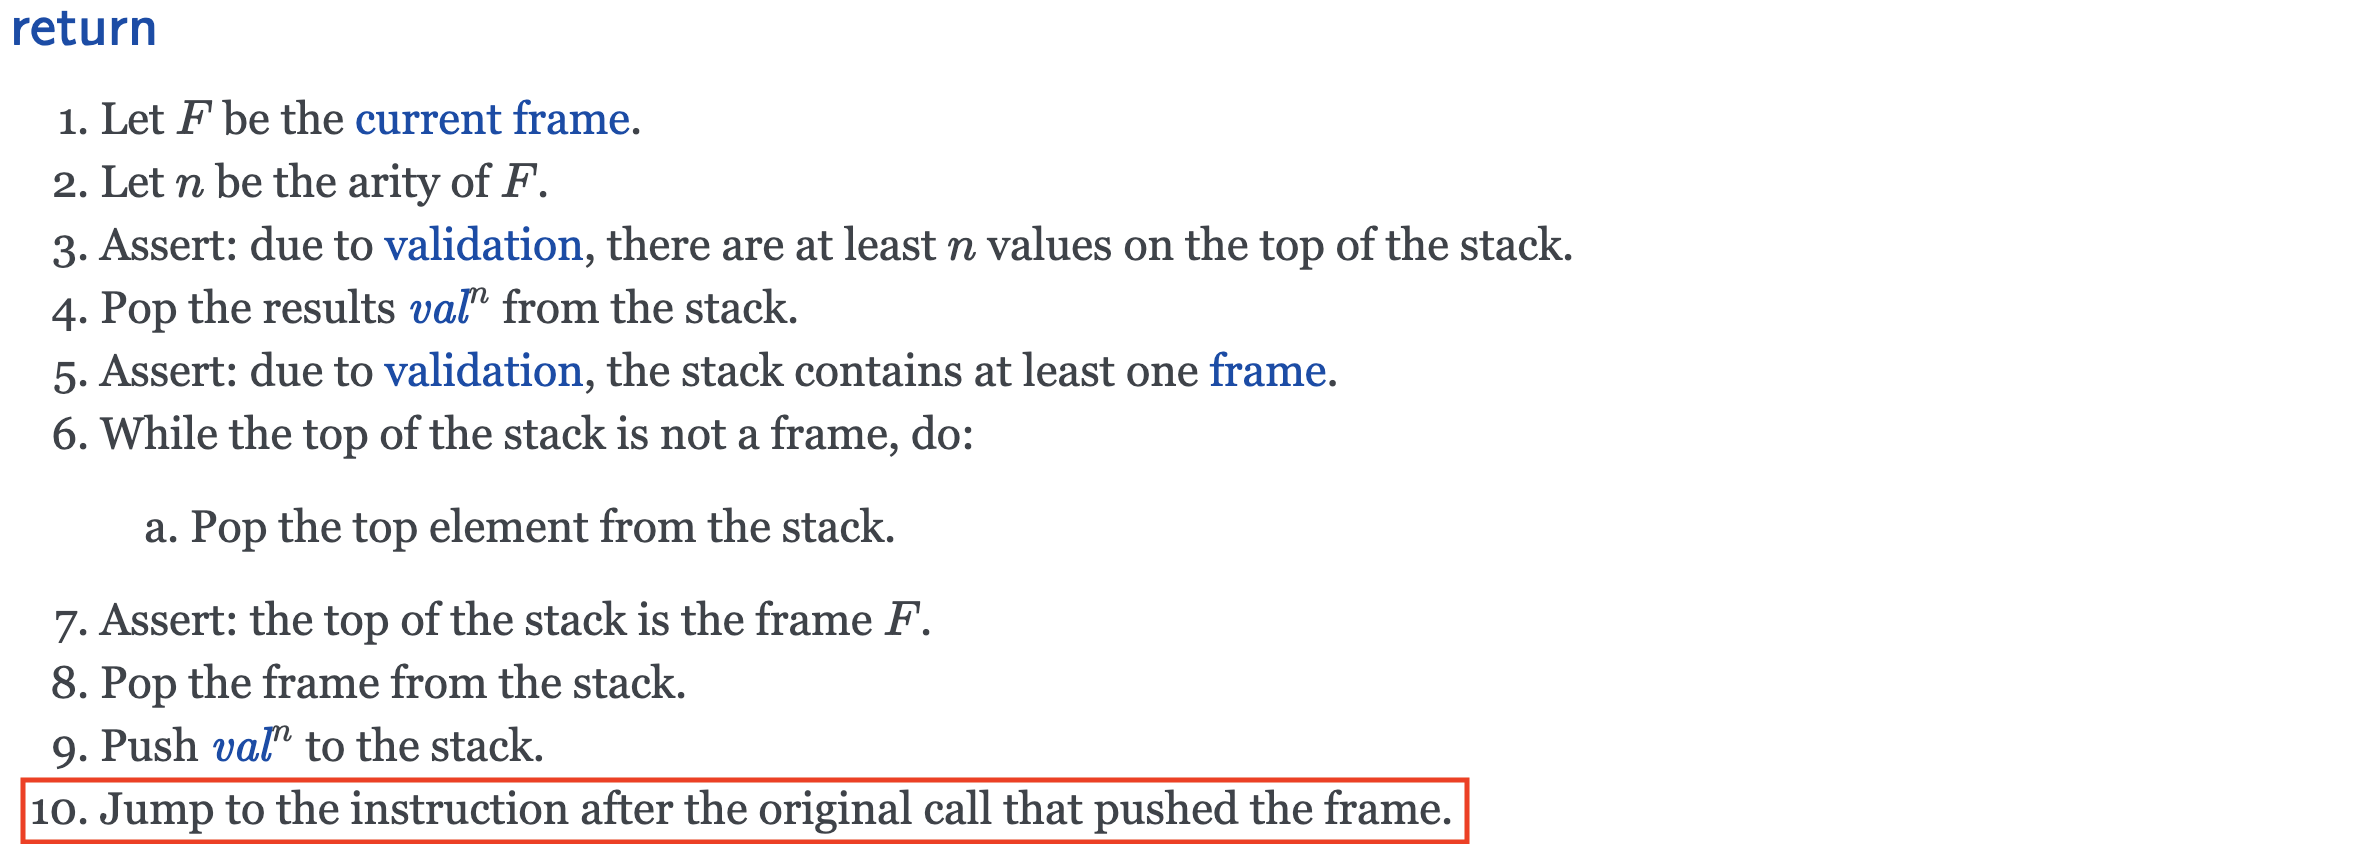
\includegraphics[width=15cm]{fig/return}}
  \caption[\texttt{return} instruction]{\texttt{return} instruction}
    \label{fig:return}
  \centerline{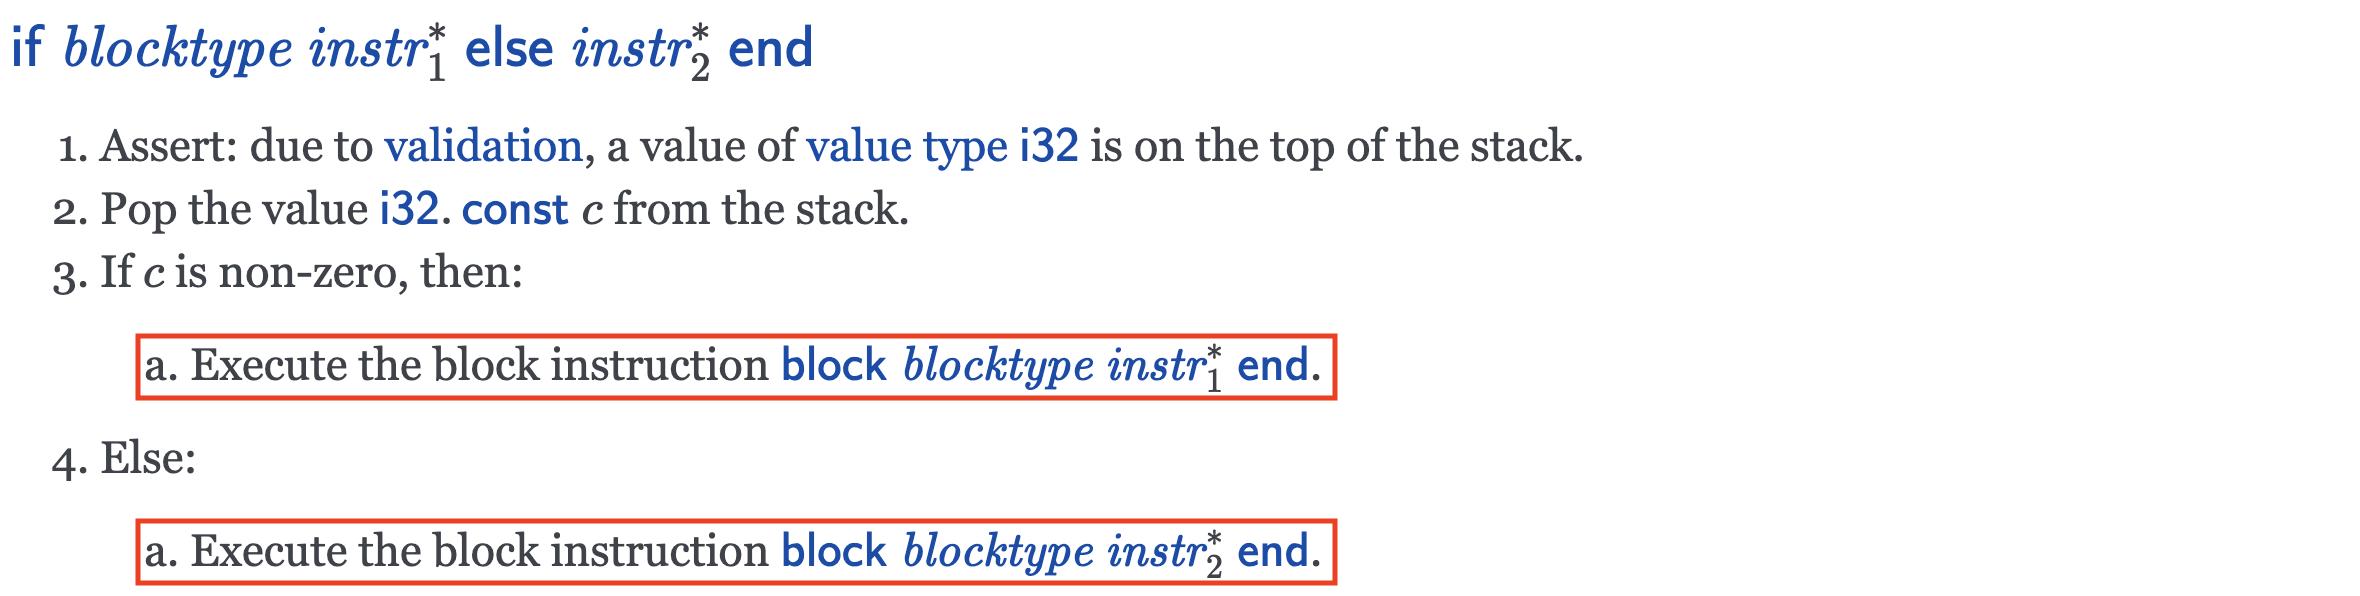
\includegraphics[width=15cm]{fig/if}}
  \caption[\texttt{if} instruction]{\texttt{if} instruction}
    \label{fig:if}
  \centerline{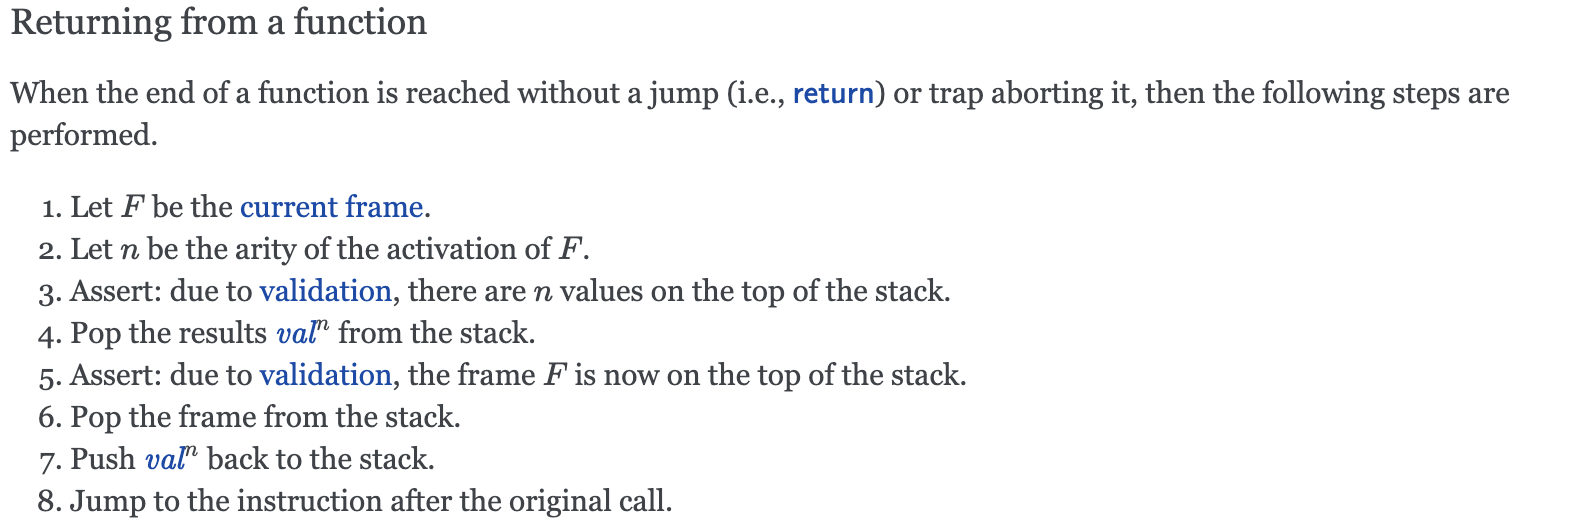
\includegraphics[width=15cm]{fig/returning}}
  \caption[Behavior for the end a block]{Behavior for the end of a block}
    \label{fig:exiting-label}
\end{figure}





\section{Definition of Algorithmic Specification Language}
\label{sec:definition}

% TODO: remove seq command
\newcommand{\seq}[1]{#1^*}

%% Syntax
\subsection{Syntax}
\label{syntax}

{
\renewcommand{\arraystretch}{0.97}  % Decrease row spacing locally
\begin{align*}
\begin{array}{lcccrlr}
%
% Algorithm
  \text{Algorithm}\quad& A &\ni& a &::=& ~ \rel ~ (s, \seq e, \seq i) ~ | ~ \fun ~ (s, \seq e, \seq i) \\
%
% Instruction
  \text{Instruction}\quad& I &\ni& i &::=& ~ \ifi ~ (e, \seq i, \seq i) &\quad\text{(If)} \\
    &&&& | & ~ \eitheri ~ (\seq i, \seq i) &\quad\text{(Either)} \\
    &&&& | & ~ \enteri ~ (e, e) &\quad\text{(Enter)} \\
    &&&& | & ~ \pushctxi ~ e &\quad\text{(Push Context)} \\
    &&&& | & ~ \pushi ~ e &\quad\text{(Push)} \\
    &&&& | & ~ \exiti ~ &\quad\text{(Exit)} \\
    &&&& | & ~ \popctxi ~ e &\quad\text{(Pop Context)} \\
    &&&& | & ~ \popi ~ e &\quad\text{(Pop)} \\
    &&&& | & ~ \popni ~ (e, e) &\quad\text{(Pop N)} \\
    &&&& | & ~ \popalli ~ e &\quad\text{(Pop All)} \\
    &&&& | & ~ \leti ~ (e, e) &\quad\text{(Let)} \\
    &&&& | & ~ \trapi &\quad\text{(Trap)} \\
    &&&& | & ~ \returnreli &\quad\text{(Return Relation)} \\
    &&&& | & ~ \returnfuni ~ e &\quad\text{(Return Function)} \\
    &&&& | & ~ \executei ~ e &\quad\text{(Execute)} \\
    &&&& | & ~ \calli ~ (s, s, \seq{e}) &\quad\text{(Let Call)} \\
    &&&& | & ~ \replaceframei ~ (p^+, e) &\quad\text{(Replace Frame)} \\
    &&&& | & ~ \replacestorei ~ (p^+, e) &\quad\text{(Replace Store)} \\
%
% Expression
  \text{Expression}\quad& E &\ni& e &::=& ~ \vare ~ s &\quad\text{(Variable)} \\
    &&&& | & ~ \nume ~ n &\quad\text{(Number)} \\
    &&&& | & ~ \boole ~ b &\quad\text{(Boolean)} \\
    &&&& | & ~ \fnamee ~ s &\quad\text{(Function Name)} \\
    &&&& | & ~ \liste ~ \seq e &\quad\text{(List)} \\
    &&&& | & ~ \stre ~ \seq{(s, e)} &\quad\text{(Record)} \\
    &&&& | & ~ \tupe ~ \seq e &\quad\text{(Tuple)} \\
    &&&& | & ~ \casee ~ (s, \seq e) &\quad\text{(Tagged Tuple)} \\
    &&&& | & ~ \une ~ (unop, e) &\quad\text{(Unary Operation)} \\
    &&&& | & ~ \bine ~ (binop, e, e) &\quad\text{(Binary Operation)} \\
    &&&& | & ~ \acce ~ (e, p) &\quad\text{(Access)} \\
    &&&& | & ~ \upde ~ (e, p^+, e) &\quad\text{(Update)} \\
    &&&& | & ~ \cate ~ (e, e) &\quad\text{(Concatenation)} \\
    &&&& | & ~ \compe ~ (e, e) &\quad\text{(Composition)} \\
    &&&& | & ~ \meme ~ (e, e) &\quad\text{(Membership)} \\
    &&&& | & ~ \choosee ~ e &\quad\text{(Choose)} \\
    &&&& | & ~ \lene ~ e &\quad\text{(Length)} \\
    &&&& | & ~ \iscaseofe ~ (e, s) &\quad\text{(Check Tag)} \\
    &&&& | & ~ \getcurctxe  &\quad\text{(Get Current Context)} \\
    &&&& | & ~ \ctxkinde ~ s &\quad\text{(Context Kind)} \\
    &&&& | & ~ \itere ~ (e, iter, \seq{s}) &\quad\text{(Iteration)} \\
    &&&& | & ~ \matche ~ (e, e) &\quad\text{(Match)} \\
    &&&& | & ~ \hastypee ~ (e, s) &\quad\text{(Has Type)} \\
\end{array}
\end{align*}
}

\newpage
\begin{align*}
\begin{array}{lcccrlr}
%
% Path
  \text{Path}\quad& P &\ni& p &::=& ~ \idxp ~ e ~ | ~ \slicep ~ (e, e) ~ | ~ \dotp ~ s \\
%
% Iter
  \text{Iter}\quad& Iter &\ni& iter &::=& ~ \listiter ~ | ~ \listniter ~ e ~|~ \listidxiter ~ (s, e) \\
%
% Operator
  \text{Unary Operator}\quad& Unop &\ni& unop &::=& ~ \notop ~ | ~ \minusop \\
  \text{Binary Operator}\quad& Binop &\ni& binop &::=& ~ \addop ~ | ~ \subop ~ | ~ \mulop \\
    &&&& | & \divop ~ | ~ \modop ~ | ~ \expop \\
    &&&& | & \implop ~ | ~ \equivop ~ | ~ \andop \\
    &&&& | & \orop ~ | ~ \eqop ~ | ~ \neop ~ | ~ \ltop \\
    &&&& | & \gtop ~ | ~ \leop ~ | ~ \geop \\
% Primitives
  \text{String}\quad& \mathbb S &\ni& s \\
  \text{Integer}\quad& \mathbb Z &\ni& n \\
  \text{Boolean}\quad& \mathbb B &\ni& b \\
\end{array}
\end{align*}

% algorithm
An algorithm is either an AL relation or an AL function, corresponding to the
relation and the function definitions in the DSL.
% instruction
An AL instruction is \ifi{} for conditionally choosing a branch, \eitheri{} for
nondeterministically choosing a branch, \enteri{} for entering a control
structure, \pushctxi{} for pushing a Wasm context, \pushi{} for pushing a Wasm
value, \exiti{} for exiting a control structure, \popctxi{} for popping a Wasm
context, \popi{} for popping a Wasm value, \popni{} for popping $n$ Wasm
values, \popalli{} for popping all Wasm values within a Wasm context, \leti{}
for let binding, \trapi{} for trapping, \returnreli{} for returning from an AL
relation, \returnfuni{} for returning from an AL function, \executei{} for
executing given Wasm instructions, \calli{} for an AL function call with let
binding, \replaceframei{} for replacing a frame, or \replacestorei{} for
replacing a store.
% expression
An expression is a variable, number, boolean, AL function name, list, record
(or struct), tuple, tagged tuple, unary or binary operation, data structure
access or update, list or record concatenation, membership check, element
selection, length retrieval, tag check, Wasm context retrieval, Wasm context
kind check, iteration, match relation, or type relation.


\begin{align*}
\begin{array}{lcccrlr}
%
% State
  \text{State}\quad& \Sigma &\ni& \sigma & ::=& ~ \seq a, w, k \\
%
% Wasm state
  \text{Wasm State}\quad& W &\ni& w &::=& ~ \seq{we}, \seq{wi}, sto \\
%
% Wasm Entry
  \text{Wasm Entry}\quad& WE &\ni& we &::=& ~ wv ~ | ~ wc \\
%
% Wasm Value
  \text{Wasm Value}\quad& WV &\ni& wv &::=& ~ \casev ~ (s, \seq v) \\
%
% Wasm Context
  \text{Wasm Context}\quad& WC &\ni& wc &::=& ~ \casev ~ (\text{``Label"}, \seq v) ~ | ~ \casev ~ (\text{``Frame"}, \seq v) \\
%
% Wasm Instruction
  \text{Wasm Instruction}\quad& WI &\ni& wi &::=& ~ \casev ~ (s, \seq v) \\
%
% Store
  \text{Store}\quad& Store &\ni& sto &::=& ~ \seq{(s, v)} \\
%
% Continuation
  \text{Continuation}\quad & K &\ni& k &::=& ~ \mt &\quad\text{(Empty)} \\
    &&&& | & ~ \toplevelcall ~ (s, \seq v) &\quad\text{(Top-level Call)} \\
    &&&& | & ~ \call ~ (s, s, \seq v, k) &\quad\text{(Call)} \\
    &&&& | & ~ \exe ~ (\seq{wi}, k) &\quad\text{(Execute)} \\
    &&&& | & ~ \wasm ~ (\seq{wc}, k) &\quad\text{(Wasm)} \\
    &&&& | & ~ \algo ~ c &\quad\text{(Algorithm)} \\
    &&&& | & ~ \ret ~ (v, k) &\quad\text{(Return)} \\
%
% Context
  \text{Context}\quad& C &\ni& c &::=& ~ (\seq i, \mu, \seq{wc}, k) \\
%
% Environment
  \text{Environment}\quad& M &\ni& \mu &::=& ~ \seq{[s \mapsto v]} \\
\end{array}
\end{align*}

\newpage
\begin{align*}
\begin{array}{lcccrlr}
%
% Value
  \text{Value}\quad& V &\ni& v &::=& ~ \numv ~ n &\quad\text{(Number)} \\
    &&&& | & ~ \boolv ~ b &\quad\text{(Boolean)} \\
    &&&& | & ~ \fnamev ~ s &\quad\text{(Function Name)} \\
    &&&& | & ~ \listv ~ \seq v &\quad\text{(List)} \\
    &&&& | & ~ \strv ~ \seq{(s, v)} &\quad\text{(Record)} \\
    &&&& | & ~ \tupv ~ \seq v &\quad\text{(Tuple)} \\
    &&&& | & ~ \casev ~ (s, \seq v) &\quad\text{(Tagged Tuple)} \\
    &&&& | & ~ \trapv &\quad\text{(Trap)} \\
    &&&& | & ~ \storev &\quad\text{(Store)} \\
\end{array}
\end{align*}

% State
An AL state consists of a sequence of algorithms, a Wasm state, and a
continuation.
% Wasm State
A Wasm state consists of an interleaved stack, a Wasm instruction stack, and a
store.
% Wasm Entry
An interleaved stack contains two types of entries: a Wasm value and a Wasm
context.
% Wasm Value & Wasm Context & Wasm Instruction
Each of a Wasm value, a Wasm context, and a Wasm instruction is expressed as an
AL value $\casev$.
In particular, the tag of a Wasm context is either ``Label" or ``Frame".
% Store
A store is expressed as a sequence of pairs, each consisting of a field name
and an AL value.
% Continuation
A continuation is \mt{} for an empty continuation, \toplevelcall{} for
top-level function call, \call{} for a function call with let binding, \exe{}
for executing given Wasm instructions, \wasm{} for executing a Wasm instruction
in the instruction stack, \algo{} for interpreting AL instructions in an
algorithm, or \ret{} for returning from an AL function.
% Env
An environment is a finite mapping from variable names to AL values.
% Context
An AL context consists of a sequence of Wasm instruction, an environment, a
sequence of Wasm contexts, and a continuation.
% Value
An AL value is a number, boolean, function name, list, record, tuple, tagged tuple,
trap, or store.


% Terminology
In this section, AL-specific terms (state, context, value, function, and
instruction) are referred to simply as state, context, value, function, and
instruction, while Wasm terms remain unchanged.




\newpage
%% Semantics
\subsection{Semantics}
\label{semantics}

%% Continuation

\begin{gather*}
\boxed{\leadsto \subseteq \Sigma \times \Sigma} \\
%
% TopLevelCall
\newline \\
  \\
  \hline
  (\seq{a}, w, \toplevelcall ~ (s, \seq v)) \leadsto (\seq{a}, w, \createalgo(\seq a, s, \seq v, \mt)) \\
%
% Call
\newline \\
  \\
  \hline
  (\seq{a}, w, \call ~ (s_{var}, s_{name}, \seq v, k)) \leadsto
  (\seq{a}, w, \createalgo(\seq a, s_{name}, \seq v, \call ~ (s_{var}, s_{name}, \seq v, k))) \\
%
% Execute-empty
\newline \\
  \\
  \hline
  (\seq{a}, w, \exe ~ (\epsilon, k)) \leadsto (\seq{a}, w, k) \\
%
% Execute-instr
\newline \\
  \casev ~ (s, \seq v) = wi \\
  \hline
  (\seq{a}, w, \exe ~ (wi ~ \seq{wi}, k)) \leadsto
  (\seq{a}, w, \createalgo(\seq a, s, \seq v, \exe ~ (\seq{wi}, k))) \\
%
% Wasm-empty
\newline \\
  \\
  \hline
  (\seq{a}, w, \wasm ~ (\epsilon, k)) \leadsto (\seq{a}, w, k) \\
%
% Wasm-instr
\newline \\
  (w', \casev ~ (s, \seq v)) = \popwasminstr(w) \\
  \hline
  (\seq{a}, w, \wasm ~ (wc^+, k))
  \leadsto
  (\seq{a}, w', \createalgo(\seq a, s, \seq v, \wasm ~ (wc^+, k))) \\
%
% Al-empty
\newline \\
  \\
  \hline
  (\seq{a}, w, \algo ~ (\epsilon, \mu, \seq{wc}, k)) \leadsto (\seq{a}, w, k) \\
%
% Al-instr
\newline \\
  \seq{a}, w, (\seq{i_1}, \mu, \seq{wc}, k) \vdash i_0 \Rightarrow (w', k') \\
  \hline
  (\seq{a}, w, \algo ~ (i_0 ~ \seq{i_1}, \mu, \seq{wc}, k)) \leadsto (\seq{a}, w', k') \\
%
% Return
\newline \\
  \mu = \getenv(c) \qquad c' = \setenv(c, \mu[s_{var} \mapsto v]) \\
  \hline
  (\seq{a}, w, \ret ~ (v, \call ~ (s_{var}, s_{name}, \seq v, \algo ~ c)) \leadsto
  (\seq a, w, \algo ~ c') \\
\end{gather*}

The semantics of AL is defined by a state transition system.
% TopLevelCall
Given algorithms $\seq a$ generated from the DSL and a Wasm state $w$, a
top-level function $s$ can be invoked with arguments $\seq v$ to perform
either module instantiation or function invocation:
$(\seq a, w, \toplevelcall ~ (s, \seq v))$.
$\toplevelcall ~ (s, \seq v)${} transitions to \algo{} with the function name
$s$, the arguments $\seq v$, and \mt{}.
% Empty
\mt{} is an empty continuation, representing the end of the transition, so no
further transition occurs.
% Call
Similarly to the top-level call, $\call~ (s_{var}, s_{name}, \seq v, k)${}
transitionsto \algo{} with the function name $s_{name}$ and the arguments $\seq
v$, but with the current continuation nested within it.
% Execute
$\exe ~ (\seq{wi}, k)${} executes each Wasm instruction in the sequence
$\seq{wi}$ one by one, each containing a relation name and arguments.
The continuation transitions to \algo{} with the relation name, the arguments,
and the current continuation, with the Wasm instruction being popped.
% Wasm
In $\wasm ~ (\seq{wc}, k)${}, a Wasm instruction is popped from
the Wasm instruction stack and executed until the Wasm context sequence
$\seq{wc}$ is exhausted.
This execution transitions the continuation to \algo{}, with the relation name
and the arguments of the Wasm instruction, and the current continuation nested
within it.
% Algo
In $\algo ~ (\seq i, \mu, \seq{wc}, k)${}, the body instructions $\seq i$
execute sequentially, allowing transitions to \call{}, \exe{}, \wasm{}, \ret{},
or \algo{}.
% Return
The execution of a function call concludes with a return instruction, which
changes the continuation to $\ret ~ v${}.
If the function call originates from \call{}, the return value $v$ is assigned
to the variable $s_{var}$.
If it originates from \toplevelcall{}, the inner continuation $k$ is always
\mt, so the entire execution concludes with the return value $v$:
$
(\seq a, w, \toplevelcall ~ (s, \seq v))
\leadsto^*
(\seq a, w', \ret ~ (v, \mt))
$.




%% Instruction

\begin{gather*}
  \boxed{\seq{a}, ~ w, ~ c \vdash i \Rightarrow w, ~ k} \\
%
% If-true
\newline \\
  w, \getenv(c) \vdash e \Rightarrow v \qquad
  \istrue(v) \\
  \hline
  \seq{a}, w, c \vdash \ifi ~ (e, \seq{i_1}, \seq{i_2}) \Rightarrow
  (w, \algo ~ (\prependinstr(c, \seq{i_1}))) \\
%
% If-false
\newline \\
  w, \getenv(k) \vdash e \Rightarrow v \qquad
  \neg \istrue(v) \\
  \hline
  \seq{a}, w, c \vdash \ifi ~ (e, \seq{i_1}, \seq{i_2}) \Rightarrow
  (w, \algo ~ (\prependinstr(c, \seq{i_2}))) \\
%
% Either-1
\newline \\
  \\
  \hline
  \seq{a}, w, c \vdash \eitheri ~ (\seq{i_1}, \seq{i_2}) \Rightarrow
  (w, \algo ~ (\prependinstr(c, \seq{i_1}))) \\
%
% Either-2
\newline \\
  \\
  \hline
  \seq{a}, w, c \vdash \eitheri ~ (\seq{i_1}, \seq{i_2}) \Rightarrow
  (w, \algo ~ (\prependinstr(c, \seq{i_2}))) \\
%
% Enter
\newline \\
  (\seq{we}, \seq{wi}, sto) = w \qquad
  (i^*, \mu, wc_1 ~ ... ~ wc_n, k) = c \\
  w, \mu \vdash e_1 \Rightarrow wc \qquad
  w, \mu \vdash e_2 \Rightarrow \listv ~ \seq{wi_1} \\
  wi = \casev ~ (\text{"End"}, wc) \qquad
  wi_1 = \casev ~ (\text{"End"}, wc_1) \quad ... \quad wi_n = \casev ~ (\text{"End"}, wc_n) \\
  wi_2^* = wi_1^* ~ wi ~ wi_1 ~ ... ~ wi_n \\
  \hline
  \seq{a}, w, c \vdash \enteri ~ (e_1, e_2)
  \Rightarrow
  (
    (wc ~ \seq{we}, wi_2^* ~ \seq{wi}, sto),
    \wasm ~ (wc ~ wc_1 ~ ... ~ wc_n, \algo ~ (i^*, \mu, \epsilon, k))
  ) \\
%
% PushCtx
\newline \\
  w, \getenv(c) \vdash e \Rightarrow wc \\
  \hline
  \seq{a}, w, c \vdash \pushctxi ~ e
  \Rightarrow
  (\push(w, wc), \algo ~ (\addctx(c, wc))) \\
%
% Push
\newline \\
  w, \getenv(c) \vdash e \Rightarrow wv \\
  \hline
  \seq{a}, w, c \vdash \pushi ~ e \Rightarrow (\push(w, wv), \algo ~ c) \\
\end{gather*}
\newpage
\begin{gather*}
%
% Exit
\newline \\
  (\seq{we}, \seq{wi}, sto) = w \qquad
  (\seq{wv}, wc, \seq{we'}) = \splitctx(\seq{we}) \\
  \seq{wi'} = \exit(\seq{wi}) \qquad
  c' = \popwasmctx_{C}(c) \\
  \hline
  \seq{a}, w, c \vdash \exiti
  \Rightarrow
  ((\seq{we'}, \seq{wi'}, sto), \algo ~ c') \\
%
% PopCtx
\newline \\
  (\seq{we}, \seq{wi}, sto) = w \qquad
  (\seq{wv}, wc, \seq{we'}) = \splitctx(\seq{we}) \\
  \mu = \getenv(c) \cdot \assign(e, wc) \qquad
  c' = \popwasmctx_{C}(c) \\
  \hline
  \seq{a}, w, c \vdash \popctxi ~ e
  \Rightarrow
  ((\seq{wv} ~ \seq{we'}, \seq{wi}, sto), \algo ~ (\setenv(c', \mu))) \\
%
% Pop
\newline \\
  (w', wv) = \pop(w) \qquad
  \mu' = \getenv(c) \cdot \assign(e, wv) \\
  \hline
  \seq{a}, w, c \vdash \popi ~ e \Rightarrow (w', \algo ~ (\setenv(c, \mu'))) \\
%
% PopN
\newline \\
  \mu = \getenv(c) \qquad
  w, \mu \vdash e_2 \Rightarrow \numv ~ n \\
  (w', wv^n) = \popn(w, n) \qquad
  \mu' = \mu \cdot \assign(e_1, \listv ~ wv^n) \\
  \hline
  \seq{a}, w, c \vdash \popni ~ (e_1, e_2) \Rightarrow
  (w', \algo ~ (\setenv(c, \mu'))) \\
%
% PopAll
\newline \\
  (\seq{wv}, wc, \seq{we'}) = \splitctx(\seq{we}) \qquad
  \mu' = \getenv(c) \cdot \assign(e, \liste ~ \seq{wv}) \\
  \hline
  \seq{a}, (\seq{we}, \seq{wi}, sto), c \vdash \popalli ~ e
  \Rightarrow
  ((wc ~ \seq{we'}, \seq{wi}, sto), \algo ~ (\setenv(c, \mu'))) \\
%
% Let
\newline \\
  \mu = \getenv(c) \qquad
  w, \mu \vdash e_2 \Rightarrow v \qquad
  \mu' = \mu \cdot \assign(e_1, v) \\
  \hline
  \seq{a}, w, c \vdash \leti ~ (e_1, e_2)
  \Rightarrow
  (w, \setenv(c, \mu')) \\
%
% Trap
\newline \\
  \\
  \hline
  \seq{a}, w, c \vdash \trapi \Rightarrow (w, \ret ~ (\trapv, \mt)) \\
%
% Return-rule
\newline \\
  \\
  \hline
  \seq{a}, w, (\seq{i}, \mu, wc^*, k) \vdash \returnreli \Rightarrow (w, k) \\
%
% Return-func
\newline \\
  w, \mu \vdash e \Rightarrow v \\
  \hline
  \seq{a}, w, (\seq{i}, \mu, wc^*, k) \vdash \returnfuni ~ e \Rightarrow
  (w, \ret ~ (v, k)) \\
%
% Execute
\newline \\
  w, \getenv(c) \vdash e \Rightarrow \listv ~ wi^* \\
  \hline
  \seq{a}, w, c \vdash \executei ~ e \Rightarrow
  (w, \exe ~ (wi^*, \algo ~ c)) \\
%
% Call-fname
\newline \\
  \mu = \getenv(c) \qquad
  \fnamev ~ s_3 = \mu(s_2) \qquad
  w, \mu \vdash e_1 \Rightarrow v_1 \quad ... \quad
  w, \mu \vdash e_n \Rightarrow v_n \\
  \hline
  \seq{a}, w, c \vdash \calli ~ (s_1, s_2, e_1 ~ ... ~ e_n) \Rightarrow
  (w, \call ~ (s_1, s_3, v_1 ~ ... ~ v_n, \algo ~ c)) \\
%
% Call-fname
\newline \\
  \mu = \getenv(c) \qquad
  s_2 \not\in \domain(\mu) \qquad
  w, \mu \vdash e_1 \Rightarrow v_1 \quad ... \quad
  w, \mu \vdash e_n \Rightarrow v_n \\
  \hline
  \seq{a}, w, c \vdash \calli ~ (s_1, s_2, \seq e) \Rightarrow
  (w, \call ~ (s_1, s_2, v_1 ~ ... ~ v_n, \algo ~ c)) \\
%
% Replace-frame
\newline \\
  \mu = \getenv(c) \qquad
  \casev ~ (\text{``Frame"}, v_1 ~ v_2) = \getcurframe(w) \qquad
  w, \mu \vdash e \Rightarrow v \\
  wc = \casev ~ (\text{``Frame"}, v_1 ~ \update(w, \mu, v_2, p^+, v)) \\
  \hline
  \seq{a}, w, c \vdash \replaceframei ~ (p^+, e) \Rightarrow
  (\setcurframe(w, wc), \algo ~ c) \\
%
% Replace-store
\newline \\
  \mu = \getenv(c) \qquad
  w, \mu \vdash e \Rightarrow v \\
  \strv ~ sto = \update(w, \mu, \strv ~ (\getstore(w)), p^+, v) \\
  \hline
  \seq{a}, w, c \vdash \replacestorei ~ (p^+, e)
  \Rightarrow (\setstore(w, sto), c) \\
\end{gather*}

Given algorithms $\seq a$, a Wasm state $w$, and a context $c$, executing an
instruction $i$ produces an updated Wasm state and a continuation.
% If
$\ifi ~ (e, i_1^*, i_2^*)${} evaluates $e$ and branches to $\seq i_1$ if the
result is true, or $\seq i_2$ otherwise.
% Either
$\eitheri ~ (i_1^*, i_2^*)${} nondeterministically selects either $i_1^*$ or
$i_2^*$.
% Enter
$\enteri ~ (e_1, e_2)${} evaluates $e_1$, pushing the resulting Wasm context
$wc$ to the interleaved stack.
It then evaluates $e_2$ to obtain the Wasm instruction sequence $wi_1^*$.
Then, the end instructions of the Wasm context $wc$ and the Wasm contexts
$wc_1 ~ ... ~ wc_n$ in the context $c$ are appended to $wi_1^*$ and pushed to
the Wasm instruction stack.
Finally, it changes the continuation to
$\wasm ~ (wc ~ wc_1 ~ ... ~ wc_n, \algo ~ (i^*, \mu, \epsilon, k))${}.
% PushCtx
$\pushctxi ~ e${} evaluates $e$, pushing the resulting Wasm context $wc$ to the
interleaved stack and the context $c$.
% Push
$\pushi ~ e${} evaluates $e$, pushing the resulting value $wv$ to the
interleaved stack.
% Exit
$\exiti${} pops all Wasm values up to and including a Wasm context $wc$ from
the interleaved stack and all Wasm instructions up to and including an end
instruction from the Wasm instruction stack.
It also pops a Wasm context from the context $c$.
% PopCtx
$\popctxi ~ e${} pops a Wasm context $wc$ from the interleaved stack.
It also pops a Wasm context from the context $c$.
Then, it assign the Wasm context $wc$ to $e$.
% Pop
$\popi ~ e${} pops a Wasm value $wv$ from the interleaved stack and assign the
value to $e$.
% PopN
$\popni ~ (e_1, e_2)${} evaluates $e_2$ to obtain a number $n$, pops $n$ Wasm
values from the interleaved stack, and assigns the values to $e_1$.
% PopAll
$\popalli ~ e${} pops all the Wasm values up to, but not including, a
Wasm context from the interleaved stack and assign the values to $e$.
% Let
$\leti ~ (e_1, e_2)${} evaluates $e_2$ and assigns the resulting value to
$e_1$.
% Trap
\trapi{} results in $\ret ~ (\trapv{}, \mt{})$ to terminate the execution.
% ReturnRel
\returnreli{} results in the continuation $k$ in the context $c$, indicating a
return from a relation algorithm.
% ReturnFunc
$\returnfuni ~ e${} evaluates $e$ to $v$, resulting in $\ret ~ (v, k)${} where
$k$ is the continuation in the context $c$.
% Execute
\executei{} evaluates $e$ to obtain a Wasm instruction sequence $wi^*$ and
result in $\exe ~ (wi^*, \algo ~ c)${}.
% Call
$\calli ~ (s_1, s_2, e_1 ~ ... ~ e_n)${} checks if $s_2$ is bound in the
environment.
If it is, it retrieves the function name $s_3$ from the environment $\mu$;
otherwise, it uses $s_2$ as the function name.
It evaluates $\seq e$ to $v^*$, resulting in $\call ~ (s_1, s_{name}, v_1 ~ ...
~ v_n)${} where $s_{name}$ is the function name.
% ReplaceFrame
\replaceframei{} retrieves the current frame $\casev ~ (\text{``Frame"}, v_1 ~
_2)${} in the Wasm context $w$.
It then evaluates $e$ to $v$, updating the value at location $v_2$ along paths
$p^+$ to $v$.
% ReplaceFrame
\replacestorei{} evaluates $e$ to $v$, updating the value at location $\strv ~
sto$ along paths $p^+$ to v.



\newpage

%% Expression

\begin{gather*}
  \boxed{w, \mu \vdash e \Rightarrow v} \\
%
% Var
\newline \\
  v = \mu(s) \\
  \hline
  w, \mu \vdash \vare ~ s \Rightarrow v \\
%
% Num
\newline \\
  \hline
  w, \mu \vdash \nume ~ n \Rightarrow \numv ~ n \\
%
% Bool
\newline \\
  \hline
  w, \mu \vdash \boole ~ b \Rightarrow \boolv ~ b \\
%
% Fname
\newline \\
  \hline
  w, \mu \vdash \fnamee ~ s \Rightarrow \fnamev ~ s \\
%
% List
\newline \\
  w, \mu \vdash e_1 \Rightarrow v_1 \quad ... \quad
  w, \mu \vdash e_n \Rightarrow v_n \\
  \hline
  w, \mu \vdash \liste ~ e_1 ~ ... ~ e_n \Rightarrow \listv ~ v_1 ~ ... ~ v_n \\
%
% Str
\newline \\
  w, \mu \vdash e_1 \Rightarrow v_1 \quad ... \quad
  w, \mu \vdash e_n \Rightarrow v_n \\
  \hline
  w, \mu \vdash \stre ~ (s_1, e_1) ~ ... ~ (s_n, e_n) \Rightarrow
  \strv ~ (s_1, v_1) ~ ... ~ (s_n, v_n) \\
%
% Tup
\newline \\
  w, \mu \vdash e_1 \Rightarrow v_1 \quad ... \quad
  w, \mu \vdash e_n \Rightarrow v_n \\
  \hline
  w, \mu \vdash \tupe ~ e_1 ~ ... ~ e_n \Rightarrow \tupv ~ v_1 ~ ... ~ v_n \\
%
% Case
\newline \\
  w, \mu \vdash e_1 \Rightarrow v_1 \quad ... \quad
  w, \mu \vdash e_n \Rightarrow v_n \\
  \hline
  w, \mu \vdash \casee ~ (s, e_1 ~ ... ~ e_n) \Rightarrow \casev ~ (s, v_1 ~ ... ~ v_n) \\
%
% Un
\newline \\
  w, \mu \vdash e \Rightarrow v \\
  \hline
  w, \mu \vdash \une ~ (unop, e) \Rightarrow \unop(unop, v) \\
%
% Bin
\newline \\
  w, \mu \vdash e_1 \Rightarrow v_1 \qquad w, \mu \vdash e_2 \Rightarrow v_2 \\
  \hline
  w, \mu \vdash \bine ~ (binop, e_1, e_2) \Rightarrow \binop(binop, v_1, v_2) \\
%
% Acc
\newline \\
  w, \mu \vdash e \Rightarrow v \\
  \hline
  w, \mu \vdash \acce ~ (e, p) \Rightarrow \access(w, \mu, v, p) \\
%
% Upd
\newline \\
  w, \mu \vdash e_1 \Rightarrow v_1 \qquad w, \mu \vdash e_2 \Rightarrow v_2 \\
  \hline
  w, \mu \vdash \upde ~ (e_1, p^+, e_2) \Rightarrow \update(w, \mu, v_1, p^+, v_2) \\
%
% Cat
\newline \\
   w, \mu \vdash e_1 \Rightarrow \listv ~ \seq{v_1} \qquad
   w, \mu \vdash e_2 \Rightarrow \listv ~ \seq{v_2} \\
  \hline
  w, \mu \vdash \cate ~ (e_1, e_2) \Rightarrow \listv ~ (\seq{v_1} ~ \seq{v_1}) \\
%
% Comp
\newline \\
   w, \mu \vdash e_1 \Rightarrow \strv ~ \seq{(s_1, v_1)} \qquad
   w, \mu \vdash e_2 \Rightarrow \strv ~ \seq{(s_2, v_2)} \\
  \hline
  w, \mu \vdash \compe ~ (e_1, e_2) \Rightarrow \strv ~ (\seq{(s_1, v_1)} ~ \seq{(s_2, v_2)}) \\
%
% Mem
\newline \\
  w, \mu \vdash e_1 \Rightarrow v_1 \qquad
  w, \mu \vdash e_2 \Rightarrow \listv ~ \seq{v_2} \\
  \hline
  w, \mu \vdash \meme ~ (e_1, e_2) \Rightarrow \boolv ~ (v_1 \in \seq{v_2}) \\
%
% Choose
\newline \\
  w, \mu \vdash e \Rightarrow \listv ~ \seq{v} \qquad
  v \in \seq{v} \\
  \hline
  w, \mu \vdash \choosee ~ e \Rightarrow v \\
%
% Len
\newline \\
  w, \mu \vdash e \Rightarrow \listv ~ \seq{v} \\
  \hline
  w, \mu \vdash \lene ~ e \Rightarrow \numv ~ |\seq v| \\
%
% IsCaseOf
\newline \\
  w, \mu \vdash e \Rightarrow \casev ~ (s', \seq{v}) \\
  \hline
  w, \mu \vdash \iscaseofe ~ (e, s) \Rightarrow \boolv ~ (s = s') \\
%
% GetCurCtx
\newline \\
  wc = \getcurctx(w) \\
  \hline
  w, \mu \vdash \getcurctxe \Rightarrow wc \\
%
% CtxKind
\newline \\
  \casev (s', \seq v) = \getcurctx(w) \\
  \hline
  w, \mu \vdash \ctxkinde ~ s \Rightarrow \boolv ~ (s = s') \\
%
% Iter-
\newline \\
  \,~\mu(s_1) = \listv ~ (v_{11} ~ ... ~ v_{1n}) \quad ... \quad
  \mu(s_m) = \listv ~ (v_{m1} ~ ... ~ v_{mn}) \\
  \mu_1 = \mu[s_1 \mapsto v_{11}, ~ ... ~ s_m \mapsto v_{m1}] \quad ... \quad
  \mu_n = \mu[s_1 \mapsto v_{1n}, ~ ... ~ s_m \mapsto v_{mn}] \\
  w, \mu_1 \vdash e \Rightarrow v_1 \quad ... \quad
  w, \mu_n \vdash e \Rightarrow v_n \\
  \hline
  w, \mu \vdash \itere ~ (e, \listiter, s_1 ~ ... ~ s_m) \Rightarrow
  \listv ~ v_1 ~ ... ~ v_n \\
%
% Iter-n
\newline \\
  w, \mu \vdash e_2 \Rightarrow \numv ~ n \\
  \,~\mu(s_1) = \listv ~ (v_{11} ~ ... ~ v_{1n}) \quad ... \quad
  \mu(s_m) = \listv ~ (v_{m1} ~ ... ~ v_{mn}) \\
  \mu_1 = \mu[s_1 \mapsto v_{11}, ~ ... ~ s_m \mapsto v_{m1}] \quad ... \quad
  \mu_n = \mu[s_1 \mapsto v_{1n}, ~ ... ~ s_m \mapsto v_{mn}] \\
  w, \mu_1 \vdash e \Rightarrow v_1 \quad ... \quad
  w, \mu_n \vdash e \Rightarrow v_n \\
  \hline
  w, \mu \vdash \itere ~ (e_1, \listniter ~ e_2, s_1 ~ ... s_m) \Rightarrow
  \listv ~ v_1 ~ ... ~ v_n \\
%
% Iter-idx
\newline \\
  w, \mu \vdash e_2 \Rightarrow \numv ~ n \\
  \mu_1 = \mu[s_1 \mapsto \numv ~ 0, ~ ... ~ s_m \mapsto \numv ~ 0] \quad ... \quad
  \mu_n = \mu[s_1 \mapsto \numv ~ n, ~ ... ~ s_m \mapsto \numv ~ n] \\
  w, \mu_1 \vdash e \Rightarrow v_1 \quad ... \quad
  w, \mu_n \vdash e \Rightarrow v_n \\
  \hline
  w, \mu \vdash \itere ~ (e_1, \listidxiter ~ e_2, s_1 ~ ... ~ s_m) \Rightarrow
  \listv ~ v_1 ~ ... ~ v_n \\
\end{gather*}
\newpage
\begin{gather*}
%
% Match
\newline \\
  w, \mu \vdash e_1 \Rightarrow v_1 \qquad
  w, \mu \vdash e_2 \Rightarrow v_2 \\
  \hline
  w, \mu \vdash \matche ~ (e_1, e_2) \Rightarrow \boolv ~ (\match(v_1, v_2)) \\
%
% HasType
\newline \\
  w, \mu \vdash e \Rightarrow v \\
  \hline
  w, \mu \vdash \hastypee ~ (e, s) \Rightarrow \boolv ~ (\hastype(v, s)) \\
\end{gather*}

Given a Wasm state $w$ and an environment $\mu$, an expression $e$ evaluates
to a value.
% Var
$\vare ~ s${} looks up the environment $\mu$ and gets the value.
% Num Bool Fname
$\nume ~ n${}, $\boole ~ b${}, and $\fnamee ~ s${} directly reduce to $\numv ~
n${}, $\boolv ~ b${}, and $\fnamev ~ s${}, respectively.
% Tuple Case List Struct
$\liste ~ e_1 ~ ... ~ e_n${}, $\stre ~ (s_1, e_1) ~ ... ~ (s_n, e_n)${}, $\tupe
~ e_1 ~ ... ~ e_n${}, and $\casee ~ (s, e_1 ~ ... ~ e_n)${} evaluate their
sub-expressions and reduce to $\listv ~ v_1 ~ ... ~ v_n${}, $\strv ~ (s_1, v_1)
~ ... ~ (s_n, v_n)${}, $\tupv ~ v_1 ~ ... ~ v_n${}, and $\casev ~ (s, v_1 ~ ...
~ v_n)${}, respectively.
% Un Bin
$\une ~ (unop, e)${} and $\bine ~ (binop, e_1, e_2)${} evaluate their
sub-expressions and perform \unop{} and \binop{}, respectively.
% Acc
$\acce ~ (e, p)${} evaluates $e$ and accesses the resulting value $v$ using a
path $p$.
% Upd
$\upde ~ (e_1, p^+, e_2)${} evaluates $e_1$ and $e_2$ to $v_1$ and $v_2$,
updating the value at location $v_1$ along paths $p^+$ to the value $v_2$.
% Cat Comp
$\cate ~ (e_1, e_2)${} and $\compe ~ (e_1, e_2)${} each evaluate two
sub-expressions $e_1$ and $e_2$, concatenating the resulting lists and
resulting records, respectively.
% Mem
$\meme ~ (e_1, e_2)${} evaluates $e_1$ and $e_2$ to $v_1$ and $\listv ~ \seq
v_2$, and checks whether $v_1$ is a member of $\seq v_2$.
% Choose Len
$\choosee ~ e$ and $\lene ~ e${} each evaluate $e$ to the list value $\listv ~
\seq v$, choosing an element from the list and calculating the length of the
list, respectively.
% IsCaseOf
$\iscaseofe ~ (e, s)${} evaluates $e$ to the tagged tuple $\casev ~ (s', \seq
v)$ and checks whether the tag $s'$ matches $s$.
% GetCurCtx
\getcurctxe{} retrieves the current Wasm context from the interleaved stack.
% CtxKind
$\ctxkinde ~ s${} retrieves the current Wasm context $\casev ~ (s', \seq v)$
and checks whether the kind $s'$ matches $s$.
% Iter
$\itere ~ (e, iter, s^*)${} behaves differently depending on $iter$.
\listiter{} and $\listniter ~ e_2${} are essentially equivalent.
They assume that all the values mapped to the variables $\seq s$ by the
environment $\mu${} are list values with the same length $n$.
$\listniter ~ e_2${} checks whether the number $n$ matches the result of
evaluating $e_2$, while \listiter{} allows any number.
It generates a sequence of environments $\mu_1 ~ ... ~ \mu_n$ where the k-th
environment maps each variable to the k-th elements of each list.
Each environment is used to evaluate $e_1$, producing a sequence of values $v_1
~ ... ~ v_n$.
Finally, it results in $\listv ~ v_1 ~ ... ~ v_n$.
$\listidxiter ~ e_2${} behaves similarly except that the variables $\seq s$ are
unbound.
It evaluates $e_2$ to obtain $n$ and then behaves like $\listniter ~ e_2${} as
if a list of values [0 ... n-1] were bound to the variables $s^*$.
% IsValid Match HasType
$\matche ~ (e_1, e_2)${} and $\hastypee ~ (e, s)${} evaluate their
sub-expressions and perform \match{} and \hastype{}, respectively.
Note that \match{} and \hastype{} represent the match relation and the type
relation in the Wasm static semantics.
Their formalization is omitted as they are highly specific to Wasm and
excessively verbose.




%% Helper functions

\begin{align*}
%
% get_algo_name
\newline \\
  &\getalgoname(\rel ~ (s, \seq e, \seq i)) = s \\
  &\getalgoname(\fun ~ (s, \seq e, \seq i)) = s \\
%
% lookup
\newline \\
  &\lookup(\epsilon, s) = \epsilon \\
  &\lookup(a ~ \seq{a}, s) =
    \begin{cases}
      a &\quad\quad \premise{if}\quad ~ s = \getalgoname(a) \\
      \lookup(\seq{a}, s) &\quad\quad \premise{otherwise}
    \end{cases}
  \\
%
% assign
\newline \\
  &\assign(\vare ~ s, v) = [s \mapsto v] \\
  &\assign(\itere ~ (e, iter, s^*), v) = \assign(e, v) \\
  &\assign(\tupe ~ e_1 ~ ... ~ e_n, \tupv ~ v_1 ~ ... ~ v_n) =
    \assign(e_1, v_1) \cdot ~ ... ~ \cdot \assign(e_n, v_n) \\
  &\assign(\liste ~ e_1 ~ ... ~ e_n, \listv ~ v_1 ~ ... ~ v_n) =
    \assign(e_1, v_1) \cdot ~ ... ~ \cdot \assign(e_n, v_n) \\
  &\assign(\casee ~ (s, e_1 ~ ... ~ e_n), \casev ~ (s, v_1 ~ ... ~ v_n)) =
    \assign(e_1, v_1) \cdot ~ ... ~ \cdot \assign(e_n, v_n) \\
  &\assign(
    w,
    \mu,
    \stre ~ (s_1, e_1) ~ ... ~ (s_2, e_n),
    \strv ~ (s_1, v_1) ~ ... ~ (s_n, v_n)
  ) =
    \assign(e_1, v_1) \cdot ~ ... ~ \cdot \assign(e_n, v_n) \\
  &\assign(\cate ~ (\liste ~ e_1 ~ ... ~ e_m, e), \listv v_1 ~ ... ~ v_n) =
    \assign(e_1, v_1) \cdot ~ ... ~ \cdot \assign(e_m, v_m) \cdot
    \assign(e, \listv ~ v_{m+1} ~ ... ~ v_n) \\
  &\assign(\cate ~ (e, \liste ~ e_1 ~ ... ~ e_m), \listv v_1 ~ ... ~ v_n) =
    \assign(e, \listv ~ v_1 ~ ... ~ v_{n-m}) \cdot
    \assign(e_1, v_{n-m+1}) \cdot ~ ... ~ \cdot \assign(e_m, v_n) \\
%
% create_algo
\newline \\
  &\createalgo(\seq a, s, \seq v, k) =
  \algo(\seq i, \mu, \epsilon, k) \\
  &\qquad\qquad\qquad\qquad\premise{if}\quad
  (\rel ~ (s, \seq e, \seq i) \quad\lor\quad \fun ~ (s, \seq e, \seq i)) = \lookup(\seq a, s)
  \quad\land\quad
  \mu = \assign(w, [\text{``s"} \mapsto \storev], \seq e, \seq v) \\
%
% split_ctx
\newline \\
  &\splitctx(\epsilon) = (\epsilon, \epsilon, \epsilon) \\
  &\splitctx(we ~ \seq{we}) =
    \begin{cases}
      (\epsilon, wc, \seq{we})
      &\quad\quad \premise{if}\quad
      we = wc \\
      (wv ~ \seq{wv}, wc, \seq{we'})
      &\quad\quad \premise{if}\quad
      we = wv \quad\land\quad
      (\seq{wv}, wc, \seq{we'}) = \splitctx(\seq{we}) \\
    \end{cases}
  \\
%
% pop-wasm-ctx_context
\newline \\
  &\popwasmctx_{C}((\seq i, \mu, epsilon, k)) = (\seq i, \mu, \epsilon, \popwasmctx_K(k)) \\
  &\popwasmctx_{C}((\seq i, \mu, wc ~ \seq{wc}, k)) = (\seq i, \mu, wc^*, k) \\
%
\newline \\
% pop-wasm-ctx_cont-mt
  &\popwasmctx_{K}(\mt) = \epsilon \\
% pop-wasm-ctx_cont-toplevelcall
  &\popwasmctx_{K}(\toplevelcall ~ (s, v^*)) = \epsilon \\
% pop-wasm-ctx_cont-call
  &\popwasmctx_{K}(\call ~ (s_1, s_2, \seq v, k)) =
    \call ~ (s_1, s_2, \seq v, (\popwasmctx_K(k)) \\
% pop-wasm-ctx_cont-execute
  &\popwasmctx_{K}(\exe ~ (v, k)) = \exe ~ (v, (\popwasmctx_K(k)) \\
% pop-wasm-ctx_cont-wasm_0
  &\popwasmctx_{K}(\wasm ~ (\epsilon, k)) = \wasm ~ (\epsilon, \popwasmctx_{K}(k)) \\
% pop-wasm-ctx_cont-wasm_nonzero
  &\popwasmctx_{K}(\wasm ~ (wc ~ \seq{wc}, k)) = \wasm ~ (\seq{wc}, k) \\
% pop-wasm-ctx_cont-al
  &\popwasmctx_{K}(\algo ~ c) = \algo ~ (\popwasmctx_C(c)) \\
% pop-wasm-ctx_cont-ret
  &\popwasmctx_{K}(\ret ~ (v, k)) = \ret ~ (v, \popwasmctx_K(k)) \\
%
% exit
\newline \\
  &\exit(wi ~ \seq{wi}) =
    \begin{cases}
      \seq{wi} &\quad\quad \premise{if}\quad ~ wi = \casev ~ (\text{"End"}, wc) \\
      \exit(\seq{wi}) &\quad\quad \premise{otherwise} \\
    \end{cases}
  \\
%
% get_env
\newline \\
  &\getenv((\seq i, \mu, wc^*, k)) = \mu \\
%
% set_env
\newline \\
  &\setenv((\seq i, \mu, wc^*, k), \mu') = (\seq i, \mu', wc^*, k) \\
%
% prepend_instr
\newline \\
  &\prependinstr((\seq i, \mu, wc^*, k), \seq{i'}) = (\seq{i'} ~ \seq i, \mu, wc^*, k) \\
%
% add_ctx
\newline \\
  &\addctx((\seq i, \mu, wc^*, k), wc') = (\seq i, \mu, wc' ~ wc^*, k) \\
%
% get_store
\newline \\
  &\getstore((\seq{we}, \seq{wi}, sto)) = sto \\
%
% set_store
\newline \\
  &\setstore((\seq{we}, \seq{wi}, sto), sto') = (\seq{we}, \seq{wi}, sto') \\
%
% pop_wasm_instr
\newline \\
  &\popwasminstr((\seq{we}, wi ~ \seq{wi}, sto)) = ((\seq{we}, \seq{wi}, sto), wi) \\
%
% push
\newline \\
  &\push((\seq{we}, \seq{wi}, sto), we) = (we ~ \seq{we}, \seq{wi}, sto) \\
%
% pop
\newline \\
  &\pop((we ~ \seq{we}, \seq{wi}, sto)) = ((\seq{we}, \seq{wi}, sto), we) \\
%
% popn
\newline \\
  &\popn((we^n ~ \seq{we}, \seq{wi}, sto), n) = ((\seq{we}, \seq{wi}, sto), we^n) \\
%
% unop
\newline \\
  &\unop(\notop, v) =
    \begin{cases}
      \boolv ~ true &\quad\quad\premise{if}\quad ~ \istrue(v) \\
      \boolv ~ false &\quad\quad\premise{otherwise} \\
    \end{cases}
  \\
  &\unop(\minusop, \numv ~ n) = \numv ~ (-n) \\
%
% get_cur_ctx
\newline \\
  &\getcurctx((\seq{we}, \seq{wi}, sto)) =
  wc \quad\quad\premise{if}\quad ~ (\seq{wv}, wc, \seq{we'}) = \splitctx(\seq{we}) \\
%
% get_cur_frame-frame
\newline \\
  &\getcurframe((\seq{we}, \seq{wi}, sto)) =
    \begin{cases}
      wc &\quad\quad\premise{if}\quad
      (\seq{wv}, wc, \seq{we'}) = \splitctx(\seq{we}) \quad\land\quad \isframe(wc)\\
      \getcurframe(\seq{we'}) &\quad\quad\premise{if}\quad
      (\seq{wv}, wc, \seq{we'}) = \splitctx(\seq{we}) \quad\land\quad \neg \isframe(wc) \\
    \end{cases}
  \\
%
% set_cur_frame-frame
\newline \\
  &\setcurframe((\seq{we}, \seq{wi}, sto), wc_{frame})
  =
  \begin{cases}
    (\seq{wv} ~ wc_{frame} ~ \seq{we'}, \seq{wi}, sto) \\
    \qquad\qquad\qquad\quad\premise{if}\quad
    (\seq{wv}, wc, \seq{we'}) = \splitctx(\seq{we}) \quad \isframe(wc) \\
    (\seq{wv} ~ wc ~ \setcurframe(\seq{we'}, wc_{frame}), \seq{wi}, sto) \\
    \qquad\qquad\qquad\quad\premise{if}\quad
    (\seq{wv}, wc, \seq{we'}) = \splitctx(\seq{we}) \quad \neg \isframe(wc) \\
  \end{cases}
  \\
%
% access-idx
\newline \\
  &\access(w, \mu, \listv ~ \seq{v}, \idxp ~ e) = \seq{v}[n]
  \qquad\qquad\qquad~\,\quad\premise{if}\quad w, \mu \vdash e \Rightarrow \numv ~ n \\
% access-slice
  &\access(w, \mu, \listv ~ \seq{v}, \slicep ~ (e_1, e_2)) = \seq{v}[n_1: n_2]
  \quad\quad\premise{if}\quad
  w, \mu \vdash e_1 \Rightarrow \numv ~ n_1 \quad\land\quad
  w, \mu \vdash e_2 \Rightarrow \numv ~ n_2 \\
% access-dot
  &\access(w, \mu, \strv ~ ((s_0, v_0) ~ \seq{(s_1, v_1)}), \dotp ~ s) =
  \begin{cases}
    v_0 &\quad\quad\premise{if}\quad s_0 = s \\
    \access(w, \mu, \strv ~ \seq{(s_1, v_1)}, \dotp ~ s) &\quad\quad\premise{otherwise} \\
  \end{cases}
  \\
% access-store
  &\access(w, \mu, \storev, p) =\access(w, \mu, \strv ~ sto, p)
  \quad\quad\premise{if}\quad w = (\seq{we}, \seq{wi}, sto)\\
%
% update
\newline \\
  % idx
  &\update(w, \mu, \listv ~ \seq{v}, (\idxp ~ e) ~ \seq{p}, v) =
  \listv ~ (\updateidx(\seq v, n, \update(w, \mu, \seq{v}[n], \seq{p}, v))) \\
  &\qquad\qquad\qquad\qquad\qquad\qquad\qquad\qquad\qquad\qquad\qquad\qquad\qquad\qquad\qquad\qquad\qquad\qquad\qquad\qquad\premise{if}\quad
  w, \mu \vdash e \Rightarrow \numv ~ n \\
  % slice
  &\update(w, \mu, \listv ~ \seq{v}, (\slicep ~ e) ~ \seq{p}, v) =
  \listv ~ (\updateslice(\seq v, n_1, n_2, \update(w, \mu, \seq{v_i}[n_1: n_2], \seq{p}, v))) \\
  &\qquad\qquad\qquad\qquad\qquad\qquad\qquad\qquad\qquad\qquad\qquad\qquad\qquad\premise{if}\quad
  w, \mu \vdash e_1 \Rightarrow \numv ~ n_1 \quad\land\quad
  w, \mu \vdash e_2 \Rightarrow \numv ~ n_2 \\
  % dot
  &\update(w, \mu, \strv ~ \seq{(s, v)}, (\dotp ~ s') ~ \seq{p}, v)
  =
  \strv ~ (\updatedot(\seq{(s, v)}, s', \update(w, \mu, \access(v, \dotp ~ s'), \seq{p}, v))) \\
%
% update_idx
\newline \\
  &\updateidx(v_0 ~ \seq{v_1}, n, v_2) =
  \begin{cases}
    v_2 ~ \seq{v_1}
    &\quad\quad\premise{if}\quad n = 0 \\
    v_0 ~ \updateidx(\seq{v_1}, n-1, v_2)
    &\quad\quad\premise{if}\quad n > 0 \\
  \end{cases} \\
%
% update_slice
\newline \\
  &\updateslice(v_0^n ~ \seq{v_1}, 0, n, v_2^n) = v_2^n ~ \seq{v_1} \\
  &\updateslice(v_0 ~ \seq{v_1}, m, n, v_2^n) =  v_0 ~ \updateslice(\seq{v_1}, m-1, n, v_2)
  \quad\quad\premise{if}\quad m > 0 \\
%
% update_dot
\newline \\
  &\updatedot((s_0, v_0) ~ \seq{(s_1, v_1)}, s_2, v_2) =
  \begin{cases}
    (s_2, v_2) ~ \seq{(s_1, v_1)}
    &\quad\quad\premise{if}\quad s_0 = s_2 \\
    (s_0, v_0) ~ \updatedot(\seq{(s_1, v_1)}, s_2, v_2)
    &\quad\quad\premise{otherwise}
  \end{cases}
  \\
%
% is_true
\newline \\
  &\istrue(v) =
  \begin{cases}
  b &\quad\quad\premise{if}\quad v = \boolv ~ b \\
    \istrue(v_1) ~ \land ~ ... ~ \land ~ \istrue(v_n) &\quad\quad\premise{if}\quad
    v = \listv ~ v_1 ~ ... ~ v_n \\
  \end{cases} \\
%
% is_frame
\newline \\
  &\isframe(v) =
  \begin{cases}
    true
    &\quad\quad\premise{if}\quad v = \casev ~ (\text{"FRAME"}, \seq v) \\
    false &\quad\quad\premise{otherwise}\\
  \end{cases}
  \\
\end{align*}




\section{An Executable WebAssembly Specification}
\label{sec:exec-spec}

% AL spec
SpecTec translates declarative definitions in the DSL into algorithms in AL.
\cref{ex:al-testop} is the generated algorithm from \cref{ex:dsl-testop},
representing the algorithmic specification for the \texttt{testop} instruction:
\\
\begin{example}
\begin{lstlisting}[style=al]
@\textbf{Step\_pure/testop}@ nt testop {
    Assert (check_type_of_stack_top(nt))
    Pop (CONST nt c_1)
    Let c = @$\dollarcode$@testop_(nt, testop, c_1)
    Push (CONST I32 c)
}
\end{lstlisting}
  \label{ex:al-testop}
\end{example}
SpecTec generates reStructuredText code from the AL algorithms.
The upper part of \cref{fig:spectec-testop} shows the rendered result of
reStructuredText code for the \texttt{testop} instruction.


% Executable
A notable feature of AL is executability, supported by SpecTec's AL interpreter
following the syntax and the semantics of AL.
This executability allows the specification itself to be executed, enabling the
execution of the specified language, Wasm.
The execution of a Wasm program begins with two entry points: module
instantiation and function invocation, both defined within the specification as
algorithms.
Executing these algorithms performs operations for executing the Wasm program,
ultimately producing its execution result.
In this way, the execution of a Wasm program is realized by the execution of
the specification itself.


% Correctness
That is to say, the prose specification written in AL, together with the AL
interpreter, functions as a Wasm interpreter which faithfully follows the
written specification.
By testing this Wasm interpreter, we can test the specification, thereby
ensuring its correctness.
